\subsection{Evaluation the forecasting performance}
In that section, we first evaluate the quality of the forecasting step. That one depends on at least two conditions:
\begin{itemize}
\item The validity of the dynamic model we use to implement forecasting.
\item An optimal choice of the set of hyperparameters on which our algorithm depends. 
\end{itemize}
We study that two points in the following.

\subsubsection{Validation of the linear dynamic model}
\label{ssse:validation}
We proved that the linear dynamic model is sufficient to describe the dynamical behavior of signals as long as the adaptive harmonic model is relevant to describe those signals. We confirm here this theoretical result on real-life signals. To this end, we apply Algorithm~\ref{alg:extension} to a larger number of pieces of a respiratory signal. The signal is 50 minutes-long and is sampled at $\fs=100$~Hz. A zoom on a small portion of the signal is displayed in Figure~\ref{fig:tho}. From that large signal, we build a dataset of $48$ non-overlapping signals of 60 seconds, \ie~$N=6000$. 

\begin{figure}
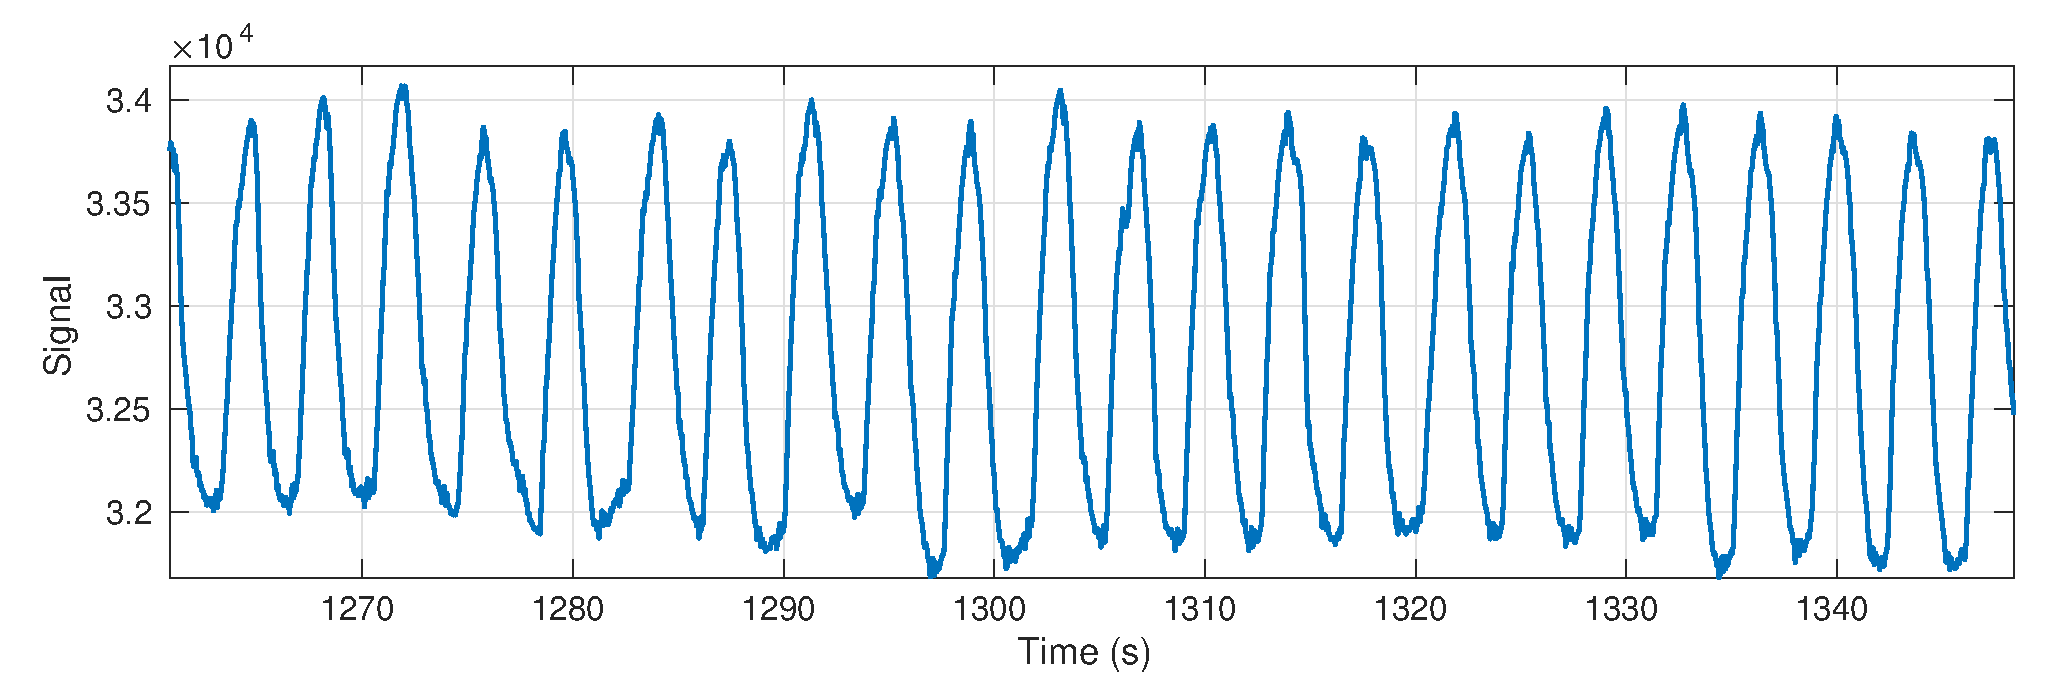
\includegraphics[width=\textwidth]{THOsig.eps}
\caption{Zoom on the respiratory signal.}
\label{fig:tho}
\end{figure}

The forecasting Algorithm~\ref{alg:extension} is applied to each of the signals in the dataset we built. These ones are extended of 7 second on each border, corresponding to $L =700$. Moreover, we choose the following set of hyperparameters: $M=\lfloor 1.5L\rfloor$ and $K=\lfloor2.5M\rfloor$. We justify such a choice in section~\ref{ssse:hyperparam}. To quantify the quality of our forecasting approach, we evaluate the Mean Square Error $\mathrm{MSE}(\tilde\bx)$ of the estimated extended signal, namely:
\[
\mathrm{MSE}(\tilde\bx) = \dfrac1{2L}\|\tilde\bx_{\rm bw} -\bx_{\rm bw}\|^2 + \dfrac1{2L}\|\tilde\bx_{\rm fw} -\bx_{\rm fw}\|^2\ .
\]
The mean and the standard deviation of the MSE with respect to the simulations are given in Table~\ref{tab:mse}. 

The results are compared with the strategy consisting in a zero-padding extension of the signal. The results neatly shows on improvement of the quality of the forecasting. Indeed, in average, the forecasting MSE is improved of almost $20\%$. Nevertheless, the variance forecasting MSE shows a huge variability in the quality of the estimation. This is probably due to the outliers and pulse that can be find in the respiratory signal. That ones make the adaptive harmonic model temporary irrelevant, and break the validity of the linear dynamic model.  

\begin{table}
\centering
\caption{Averaged MSE.}
\begin{tabular}{|c||c|c|}
  \hline
   \multirow{2}{*}{Algorithm} & \multicolumn{2}{c|}{MSE} \\
   \cline{2-3}
      & Mean & Standard deviation\\
   \hhline{|=#=|=|}
   {\sf SigExt} & $0.7935$ & $0.2615$ \\
   \hline
   Zero padding & $0.9903$ & $0.0579$ \\
   \hline
\end{tabular}
\label{tab:mse}
\end{table}

\subsubsection{Influence of the hyperparameters}
\label{ssse:hyperparam}
We evaluate the influence of the hyperparameters $K$ and $M$ on the forecasting MSE. This study is performed on a 32 second-long photoplethysmogram (PPG) signal, which is displayed on the top of Figure~\ref{fig:ppg}. This signal is sampled at $\fs=125$~Hz.

\begin{figure}
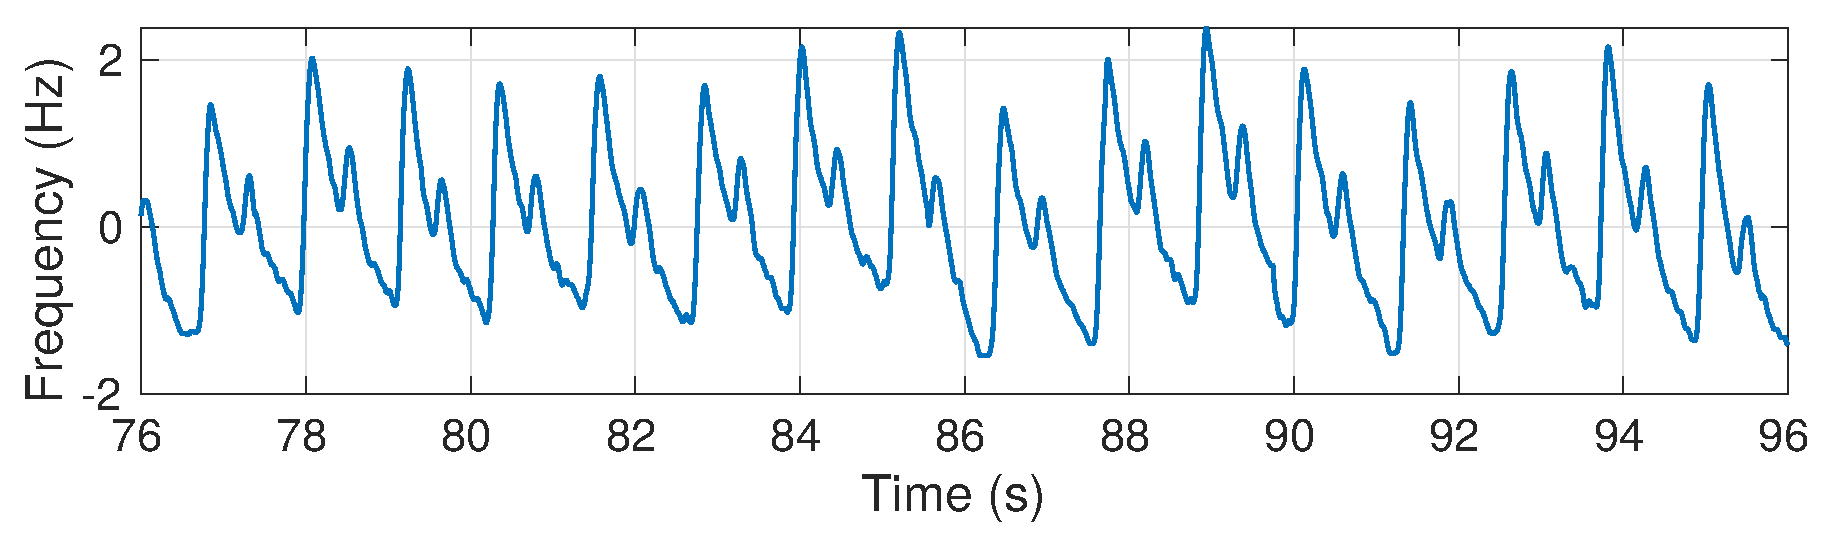
\includegraphics[width=\textwidth]{PPGsig.eps}
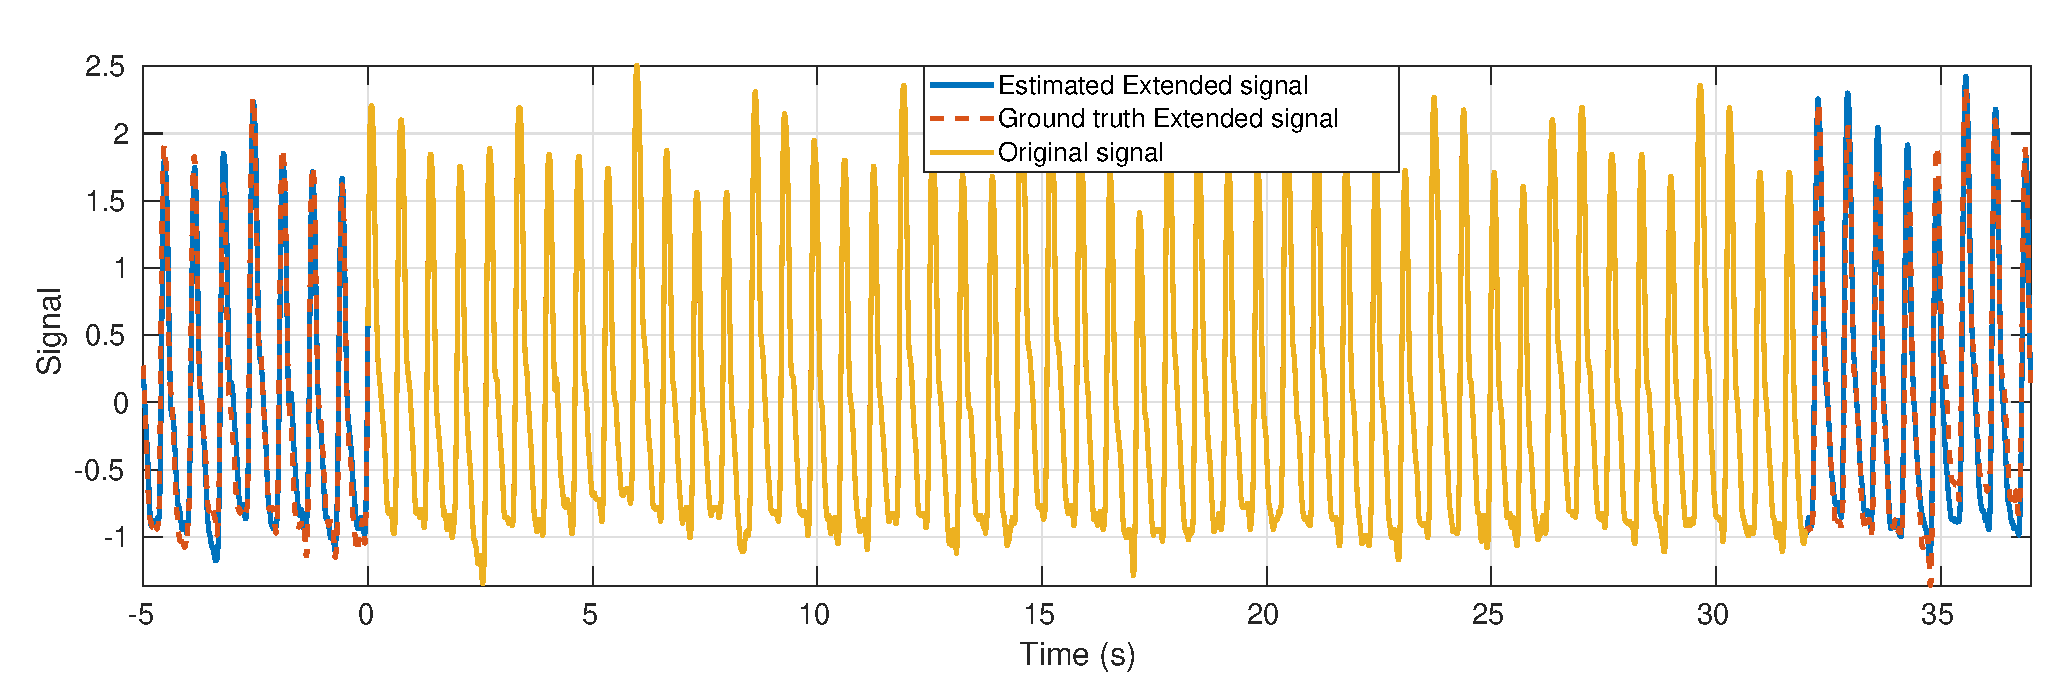
\includegraphics[width=\textwidth]{PPGforecast.eps}
\caption{PPG signal. Top: original measured signal. Extended signal obtained by forecasting superimposed with the ground truth signal.}
\label{fig:ppg}
\end{figure}

In this study, the extension length $L$ is fixed because the second step of the Algorithm~\ref{alg:boundary} determines the length $L$. Indeed, in order to avoid boundary effect, this one should be at least equal to the half of the width of the window used to perform the kernel-based transform. In practice, we choose to extend the signal if 2~seconds on each side, \ie~$L=250$.
\begin{enumerate}[a),leftmargin=*]
\item 
We perform the forecasting Algorithm~\ref{alg:extension} for different values of the sub-signals length $M$. Meanwhile, the value of $K$ is unchanged and set to $K=10L$. The graph on the left in Figure~\ref{fig:influence.M} shows the influence of $M$ on the forecasting MSE. 
%When $M$ is smaller than $L$, the forecasting algorithm cannot provide accurate forecasting because . As soon as $M$ is greater than $L$, the MSE will not be influenced by the sub-signal lengths. Indeed, the information provided by
\item
We perform the forecasting Algorithm~\ref{alg:extension} for different values of the sub-signals dataset size $K$, when the value of $M$ is set to $M=\lfloor 1.5L\rfloor$. The graph on the left in Figure~\ref{fig:influence.M} shows the influence of $K$ on the forecasting MSE.
\end{enumerate} 

\begin{figure}
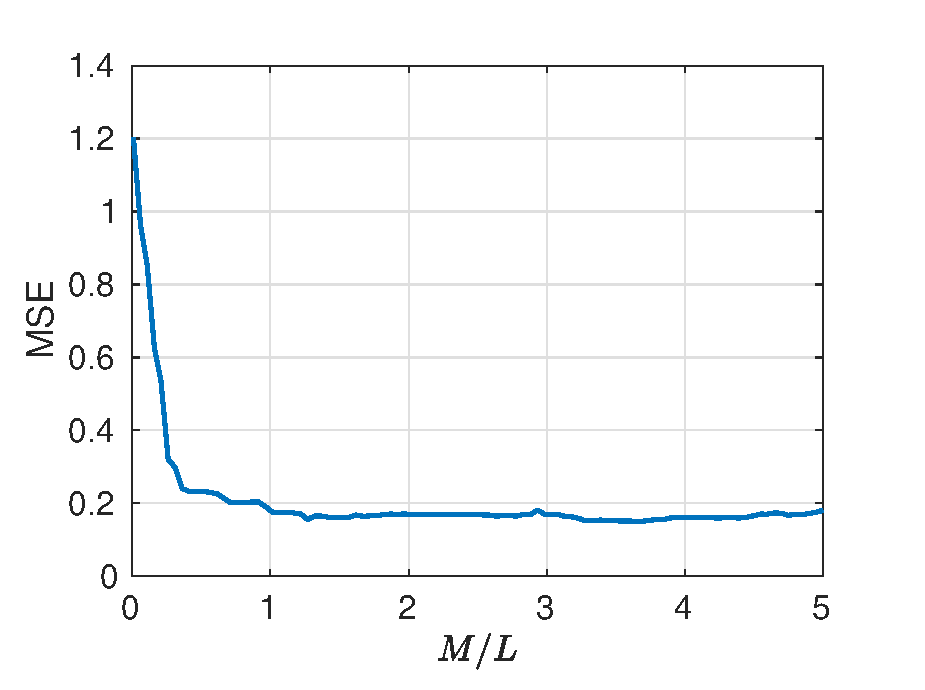
\includegraphics[width=.5\textwidth]{mseM.eps}
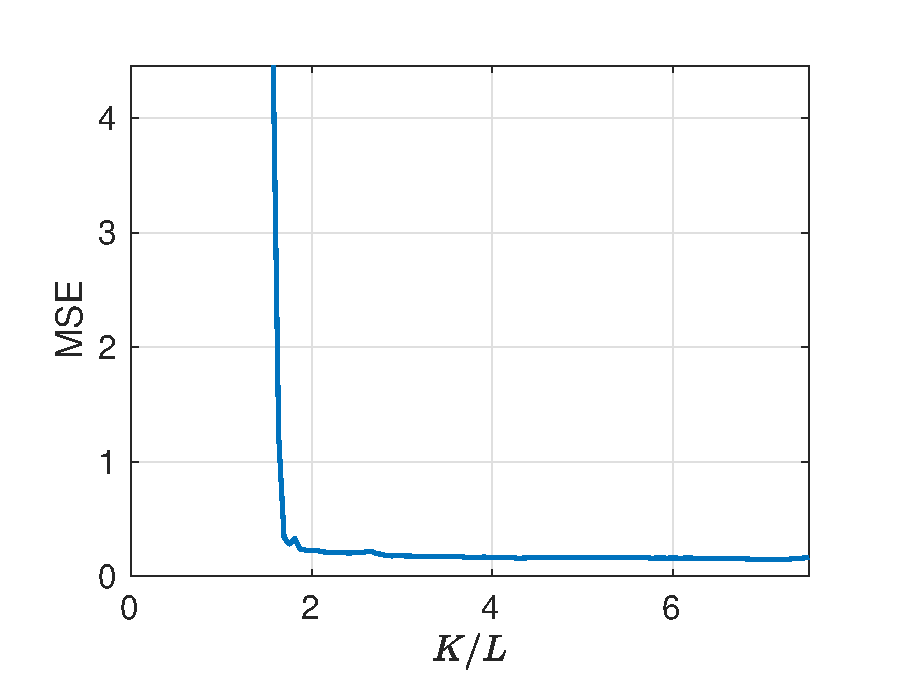
\includegraphics[width=.5\textwidth]{mseK.eps}
\caption{Influence of the size parameters on the forecasting MSE. Left: MSE in function of the sub-signals length $M$. Right: MSE in function of the sub-signal dataset size $K$.}
\label{fig:influence.M}
\end{figure}

\paragraph{Influence of noise.}
The same kind of study is done. The results are displayed on Figure~\ref{fig:influence.noise}. Here, $M=\lfloor 1.5L\rfloor$ and $K=2M$.

\begin{figure}
\centering
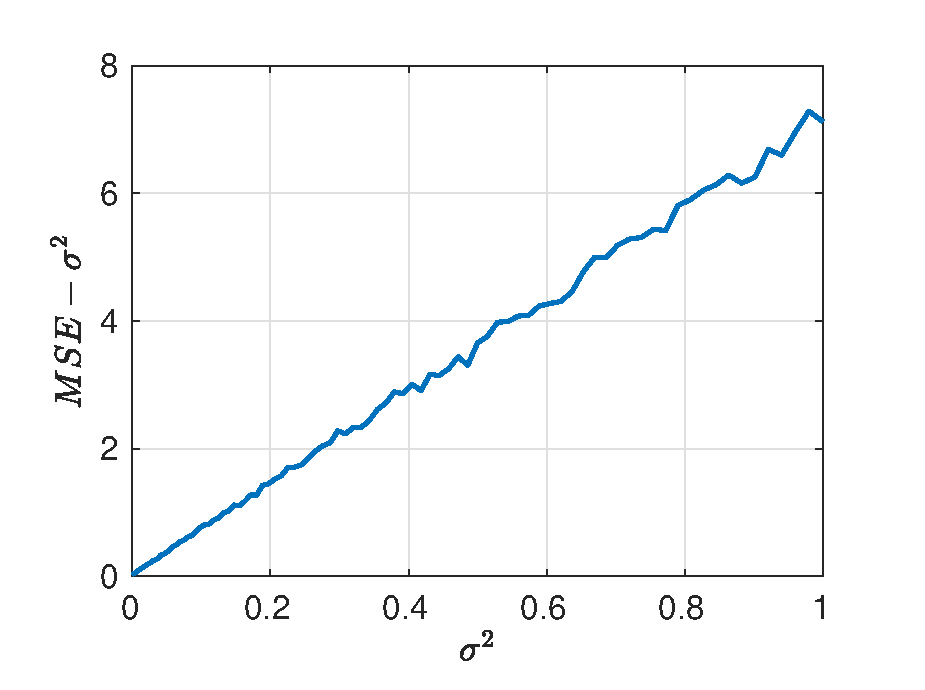
\includegraphics[width=.7\textwidth]{mseNoise.eps}
\caption{Influence of the noise variance on the forecasting MSE.}
\label{fig:influence.noise}
\end{figure}

\subsection{Evaluation of the quality of the boundary effect reduction}
The quality of the boundary effect reduction step must be evaluated of the synchrosqueezing representation. To that aim, we compare the obtained synchrosqueezing transform to the optimal synchrosqueezing transform $\ccF_N^\mathrm{opt}(\bx)$. The optimal synchrosqueezing transform is defined as the restriction of the synchrosqueezing of the ground truth extended signal $\bx^\mathrm{ext} = \begin{pmatrix}\bx[-L] & \cdots & \bx[N-1+L] \end{pmatrix}$. Therefore:
\begin{equation*}
\ccF_N^\mathrm{opt}(\bx) = \cR\left( \ccF_{N+2L}(\bx^\mathrm{ext}) \right) \ .
\end{equation*} 

The different representations we obtained must be compared to the optimal SST. To that aim, we establish a criterion that quantify the distance of these time-frequency representations to the optimal one. To do this, we reason in analogy with the optimal transport distance which allows us to quantify the distance between two probability density functions. Let us generically denote a time frequency representation $\ccQ$. Then, for $t$ fixed, we consider the following pseudo probability density function:
\begin{align}
p_\ccQ^t(\xi) &= \dfrac{|\ccQ(\xi,t)|^2}{\int_\RR |\ccQ(\nu,t)|^2\dd\nu}\ .
\label{eq:ppdf}
\end{align}
Similarly, let $p_{\ccF_0}^t$ denotes the associated pseudo-probability density function (defined as in~\eqref{eq:ppdf}) associated with the reference time-frequency representation $\ccF_0$. At each instant $t$, we can then determine the optimal transport distance $d_{t}$ between the two pseudo densities. It is given by the $L^1$ norm of the difference between the associated distribution functions. In other words, either $P_{\ccQ}^t(\xi)=\int_{-\infty}^\xi p_{\ccQ}^t(\nu)\dd\nu$ and $\tilde P_{\ccF_0}^t(\xi)=\int_{-\infty}^\xi\tilde p_{\ccF_0}^t(\nu)\dd\nu$, we have
\begin{equation*}
d_{t}(\ccQ,\ccF_0) = \int_\RR\left|\tilde P_{\ccQ}^t(\xi)-  P_{\ccF_0}^t(\xi)\right|\dd\xi\ .
\end{equation*}
Finally, the distance between the two time-frequency representations is obtained by averaging all the optimal transport distances with respect to time:
\begin{equation}
D(\ccQ,\ccF_0) = 100\times\frac1{|I|}\int_I d_{t}(\ccQ,\ccF_0)\dd t\ .
\end{equation}
The \textit{Optimal Transport Distance} (OTD) quantifies the proximity between the estimated and actual instantaneous frequencies while favouring the sparsity of the estimated time-frequency representation.

This distance is evaluated on the dataset of respiratory signals introduced in section~\ref{ssse:validation}. The results are summarize in Table~\ref{tab:otd}. The OTD averaged over the simulations clearly shows that $\ccF_\mathrm{FC}$ outperforms $\ccF$. This highlights the ability of our approach to limit the distortion due the boundary effect and provide a more accurate synchrosqueezing transform. Moreover, the OTD decreases by almost $50\%$ from the standard SST $\ccF$ to the improved SST $\ccF_{\mathrm{FC}}$. Thus, the improvement obtained by forecasting in the time domain is amplified in the time-frequency domain. 

\begin{table}
\centering
\caption{Performance of the Boundary effect reduction on the SST.}
\begin{tabular}{|c||c|c|}
  \hline
   \multirow{2}{*}{Algorithm} & \multicolumn{2}{c|}{OTD to $\ccF_N^{\mathrm{opt}}(\bx)$} \\
   \cline{2-3}
      & Mean & Standard deviation\\
   \hhline{|=#=|=|}
   $\ccF_N^{\mathrm{ext}}(\bx)$ & $4.705\times 10^{-3}$ & $3.147\times 10^{-3}$ \\
   \hline
   $\ccF_N(\bx)$ & $9.195\times 10^{-3}$ & $3.453\times 10^{-3}$ \\
   \hline
\end{tabular}
\label{tab:otd}
\end{table}